\documentclass{article}
\usepackage[utf8]{inputenc}

\usepackage[paperwidth=8.5in, paperheight=11in, top=1in, bottom=.5in, left=.5in, right=.5in]{geometry}
\usepackage{fancyhdr, graphicx,tikz,amsmath,multicol,paracol}
\usepackage[inline]{enumitem}


\pagestyle{fancy}
\lhead{\large{\textbf{Module 1: Limits - Readiness Assurance Test}}}
\chead{}
\rhead{}
\lfoot{}
\cfoot{}
%\rfoot{\thepage/\pageref{LastPage} }
\setlength{\headheight}{14pt} %added in bc warning

%%% The answers are aligned to IF-AT Form B012, questions 11-20. 

% 1 D
% 2 B
% 3 C
% 4 A
% 5 D
% 6 D
% 7 C
% 8 D
% 9 B
% 10 A


\begin{document}


\begin{enumerate}




%factoring, rational expressions
    \item Simplify the following expression:
        \[  \frac{x^2+5x+6}{x^2-4}
        \]

                  \begin{multicols}{4}
                  \begin{enumerate}[label=\Alph*)]
                      \item $ \dfrac{(x-3)}{(x+2)}$
                      \item $ \dfrac{(x-3)}{(x-2)}$
                      \item $ \dfrac{(x+3)}{(x+2)}$
                      \item $ \dfrac{(x+3)}{(x-2)}$ %correct

                  \end{enumerate}
                  \end{multicols}



% number lines, inequalities, interval notation
   \item An interval is shown below on a number line.
        \begin{center}
                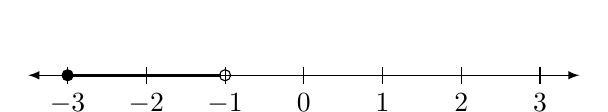
\begin{tikzpicture}
                \draw[latex-latex] (-3.5,0) -- (3.5,0) ; %edit here for the axis
                \foreach \x in  {-3,-2,-1,0,1,2,3} % edit here for the vertical lines
                \draw[shift={(\x,0)},color=black] (0pt,3pt) -- (0pt,-3pt);
                \foreach \x in {-3,-2,-1,0,1,2,3} % edit here for the numbers
                \draw[shift={(\x,0)},color=black] (0pt,0pt) -- (0pt,-3pt) node[below] 
                {$\x$};
                \draw[very thick] (-3,0) -- (-1.05,0);
                \filldraw (-3,0) circle (2pt);
                \draw (-1,0) circle (2pt);
                %\draw[very thick] (0.05,0) -- (1.95,0);
                %\filldraw (2,0) circle (2pt);
                %\draw (0,0) circle (2pt); 
                \end{tikzpicture}
            \end{center}

        A second interval is represented by the inequality $0 < x \leq 2$. 

        What is the union of these two intervals in interval notation?

                  \begin{multicols}{4}
                  \begin{enumerate}[label=\Alph*)]
                      \item $(-3,-1] \cup (0,2] $
                      \item $[-3,-1) \cup (0,2] $ %correct
                      \item $[-3,-1) \cup [0,2) $ 
                      \item $(-3,-1] \cup [0,2) $
                  \end{enumerate}
                  \end{multicols}

%polynomial multiplication
    \item Which expression is equal to the product $(x-4)(x^2+3x-3)$?

            \begin{enumerate}[label=\Alph*)]
                  
                  \item $x^2 + 4x - 7$ %added rather than multiplied
                  \item $x^3 + 7x^2 + 9x - 12$ % used 4 instead of -4
                  \item $x^3 - x^2 - 15 x + 12$ % correct
                  \item $-4x^2 - 11x + 12$ %only distributed the -4
              \end{enumerate}

% asymptotes, holes, factoring
    \item Find all vertical asymptote(s), horizontal asymptote(s), and hole(s) for the function given below.
        \[ f(x) = \frac{x^2-6x+8}{x^2-5x+6}
        \]

          \begin{enumerate}[label=\Alph*)]
              
            \item vertical asymptote of $x=3$, horizontal asymptote of $y=1$, hole when $x=2$ %correct
            \item vertical asymptote of $x=2$, horizontal asymptote of $y=1$, hole when $x=3$
          \item vertical asymptote of $x=3$, horizontal asymptote of $y=4$, hole when $x=2$ 
              \item vertical asymptote of $x=2$, horizontal asymptote of $y=4$, hole when $x=3$
              

          \end{enumerate}



%\pagebreak

%graphing, piecewise funtions, function notation, holes, inequalities
    \item Which piecewise function represents the graph below? (Assume the ends of the graphs continue in the directions they seem to.)

        \begin{multicols}{2}
        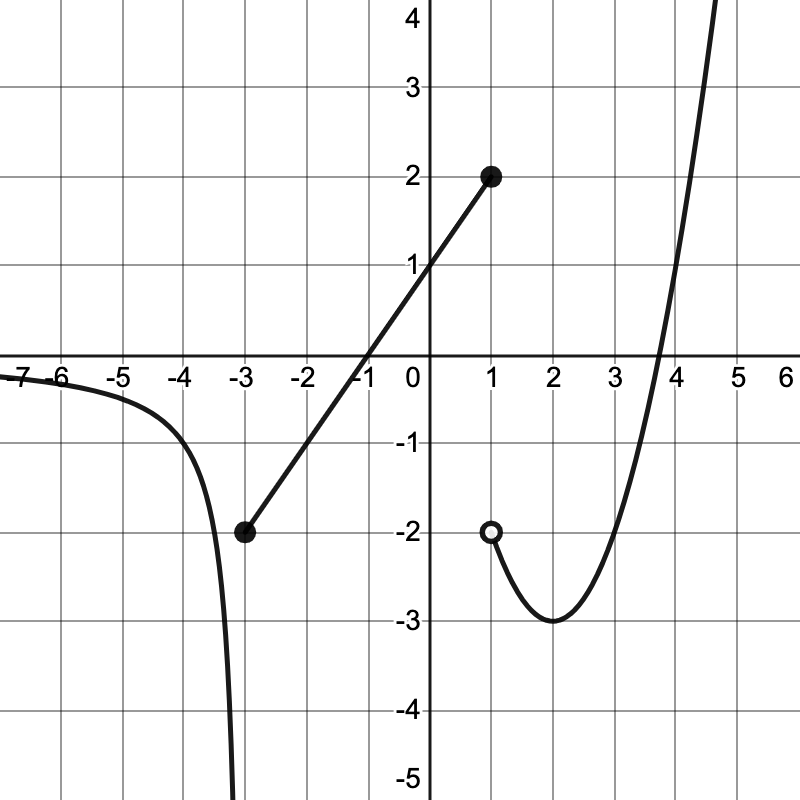
\includegraphics[scale=.25]{images/piecewise_limits_RAT.png}


        \begin{enumerate}[label=\Alph*),itemsep=5pt]


              \item $ f(x) = \begin{cases} 
                      \dfrac{1}{x+3}    & x \leq -3 \\
                      x+1               & -3 < x < 1 \\
                      x^2-4x+1          & 1 \leq x 
                      \end{cases}$ %opposite signs in each spot

              \item $ f(x) = \begin{cases} 
                      \dfrac{1}{x+3}    & x < 0 \\
                      x+1               & -2\leq x \leq 2 \\
                      x^2-4x+1          & 3 < x 
                      \end{cases}$ %used y-values, not x

              \item $ f(x) = \begin{cases} 
                      \dfrac{1}{x+3}    & x \leq 0 \\
                      x+1               & -2 < x < 2 \\
                      x^2-4x+1          & 3 \leq x 
                      \end{cases}$ %used y-values, not x
              \item $ f(x) = \begin{cases} 
                      \dfrac{1}{x+3}    & x < -3 \\
                      x+1               & -3\leq x \leq 1 \\
                      x^2-4x+1          & 1 < x 
                      \end{cases}$  %correct
            \end{enumerate}
          \end{multicols}



%domain, rational functions
    \item What is the domain of the function shown below?
    \[
       f(x) = \frac{x-1}{x+1} + \frac{x+3}{x-4}
    \]
            \begin{enumerate}[label=\Alph*)]
                %\item All real numbers
                \item All real numbers except $1$ and $-3$
                \item All real numbers except $1$ and $-4$
                \item All real numbers except $-1$ and $3$
                \item All real numbers except $-1$ and $4$ %correct
            \end{enumerate}

% function notation
     \item Suppose that $q = f(p)$, so that the quantity $q$ is a function of the quantity $p$. Let's say the dependent variable has value 10 when the independent variable has value 2. Which equation best expresses this relationship?

                  \begin{enumerate}[label=\Alph*)]
                      \item $f(p)=2$
                      \item $f(2)=p$
                      \item $10 = f(2)$ %correct
                      \item $2 = f(10)$
                      
                  \end{enumerate}


%function notation, graphing, holes
    \item Consider the function $h(x)$ whose graph is pictured below. Select the most accurate statement.
              \begin{multicols}{2}
              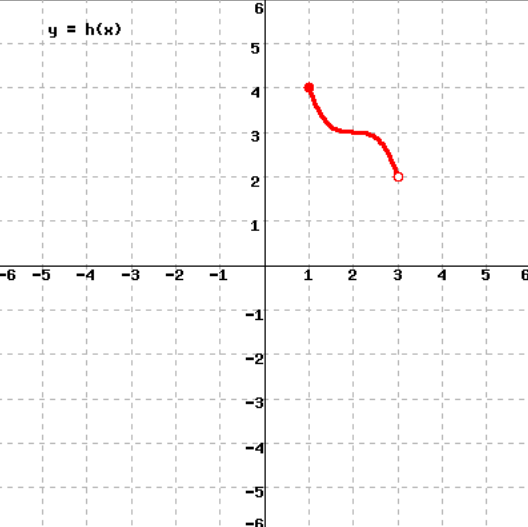
\includegraphics[keepaspectratio=True, width=0.6\linewidth]{images/eval-dom-rng.png}

              \begin{enumerate}[label=\Alph*)]
                   \item $h(4) = 1$
                   \item $h(1)$ is not defined 
                   \item $h(3) = 2$
                   \item $h(2) = 3$%correct
              \end{enumerate}
              \end{multicols}


\end{enumerate}


\end{document}
